\newpage
\appendix
\section{Code VHDL}
\todo{Finish this this}

\begin{figure}[H]
	\tiny
	\centering
	\begin{varwidth}{\linewidth}
		\begin{verbatim}
architecture Behavioral of Thermo2Bin is
    signal first_segment_of_four : STD_LOGIC_VECTOR(3 downto 0);
    signal second_segment_of_four : STD_LOGIC_VECTOR(3 downto 0);
    signal third_segment_of_four : STD_LOGIC_VECTOR(3 downto 0);

    component Add4Bits is
        Port ( A : in STD_LOGIC_VECTOR (3 downto 0);
            B : in STD_LOGIC_VECTOR (3 downto 0);
            C : in STD_LOGIC;
            R : out STD_LOGIC_VECTOR (3 downto 0);
            Rc : out STD_LOGIC);
    end component;

    signal first_plus_second : STD_LOGIC_VECTOR(3 downto 0);
    signal carry_out_first_plus_second : STD_LOGIC;
    signal last_carry_out : STD_LOGIC;

begin
    first_segment_of_four(3) <= '0';
    first_segment_of_four(2) <= thermo_bus(11);
    first_segment_of_four(1) <= NOT thermo_bus(11) AND thermo_bus(9);
    first_segment_of_four(0) <= NOT thermo_bus(11) AND ((NOT thermo_bus(9) AND thermo_bus(8)) OR (thermo_bus(10) AND thermo_bus(9)));

    second_segment_of_four(3) <= '0';
    second_segment_of_four(2) <= thermo_bus(7);
    second_segment_of_four(1) <= NOT thermo_bus(7) AND thermo_bus(5);
    second_segment_of_four(0) <= NOT thermo_bus(7) AND ((NOT thermo_bus(5) AND thermo_bus(4)) OR (thermo_bus(6) AND thermo_bus(5)));

    third_segment_of_four(3) <= '0';
    third_segment_of_four(2) <= thermo_bus(3);
    third_segment_of_four(1) <= NOT thermo_bus(3) AND thermo_bus(1);
    third_segment_of_four(0) <= NOT thermo_bus(3) AND ((NOT thermo_bus(1) AND thermo_bus(0)) OR (thermo_bus(2) AND thermo_bus(1)));

    first_plus_second_adder : Add4Bits port map (
      A => first_segment_of_four,
      B => second_segment_of_four,
      R => first_plus_second,
      Rc => carry_out_first_plus_second,
      C => '0');

    plus_third_adder : Add4Bits port map (
      A => first_plus_second,
      B => third_segment_of_four,
      R => binary_out,
      Rc => last_carry_out,
      C => carry_out_first_plus_second);

    error <= (
    (thermo_bus(11) AND NOT thermo_bus(10)) OR
    (thermo_bus(10) AND NOT thermo_bus(9)) OR
    (thermo_bus(9)  AND NOT thermo_bus(8)) OR
    (thermo_bus(8)  AND NOT thermo_bus(7)) OR
    (thermo_bus(7)  AND NOT thermo_bus(6)) OR
    (thermo_bus(6)  AND NOT thermo_bus(5)) OR
    (thermo_bus(5)  AND NOT thermo_bus(4)) OR
    (thermo_bus(4)  AND NOT thermo_bus(3)) OR
    (thermo_bus(3)  AND NOT thermo_bus(2)) OR
    (thermo_bus(2)  AND NOT thermo_bus(1)) OR
    (thermo_bus(1)  AND NOT thermo_bus(0)));

end Behavioral;
\end{verbatim}

	\end{varwidth}
	\caption{Module Thermo2bin}
\end{figure}

\begin{figure}[H]
	\tiny
	\centering
	\begin{varwidth}{\linewidth}
		\begin{verbatim}
architecture Behavioral of Add4Bits is

  signal bufA : STD_LOGIC;
  signal bufB : STD_LOGIC;
  signal bufC : STD_LOGIC;

  component Add1BitA is Port (
    X : in STD_LOGIC;
    Y : in STD_LOGIC;
    Ci: in STD_LOGIC;
    O : out STD_LOGIC;
    Co: out STD_LOGIC);
  end component;

  component Add1BitB is Port (
    X : in STD_LOGIC;
    Y : in STD_LOGIC;
    Ci: in STD_LOGIC;
    O : out STD_LOGIC;
    Co: out STD_LOGIC);
  end component;

begin

  first : Add1BitB port map (
    X  => A(0),
    Y  => B(0),
    Ci => C,
    O => R(0),
    Co => bufA);

  sec : Add1BitB port map (
    X  => A(1),
    Y  => B(1),
    Ci => bufA,
    O => R(1),
    Co => bufB);

  third : Add1BitA port map (
    X  => A(2),
    Y  => B(2),
    Ci => bufB,
    O => R(2),
    Co => bufC);

  fourth : Add1BitA port map (
    X  => A(3),
    Y  => B(3),
    Ci => bufC,
    O => R(3),
    Co => Rc);

end Behavioral;
\end{verbatim}

	\end{varwidth}
	\caption{Module Add4Bits}
\end{figure}

\begin{figure}[H]
	\tiny
	\centering
	\begin{varwidth}{\linewidth}
		\begin{verbatim}
architecture Behavioral of Add1BitA is

begin

  O  <= (X xor Y) xor Ci;
  Co <= ((X xor Y) and Ci) or (X and Y);

end;
\end{verbatim}

	\end{varwidth}
	\caption{Module Add1BitA}
\end{figure}

\begin{figure}[H]
	\tiny
	\centering
	\begin{varwidth}{\linewidth}
		\begin{verbatim}
architecture Behavioral of Add1BitB is

begin

Adder: process(X, Y, Ci) is variable buf: STD_LOGIC_VECTOR(2 downto 0);
begin
  buf(0) := X;
  buf(1) := Y;
  buf(2) := Ci;

  case (buf) is
    when "000" =>
      O  <= '0';
      Co <= '0';
    when "001" =>
      O  <= '1';
      Co <= '0';
    when "010" =>
      O  <= '1';
      Co <= '0';
    when "011" =>
      O  <= '0';
      Co <= '1';
    when "100" =>
      O  <= '1';
      Co <= '0';
    when "101" =>
      O  <= '0';
      Co <= '1';
    when "110" =>
      O  <= '0';
      Co <= '1';
    when "111" =>
      O  <= '1';
      Co <= '1';
    when others =>
      O  <= '0';
      Co <= '0';
  end case;

end process Adder;

end Behavioral;
\end{verbatim}

	\end{varwidth}
	\caption{Module Add1BitB}
\end{figure}

\section{Schémas}

\todo{Schéma bloc}\\
\todo{Simulations}


\begin{figure}[H]
	\centering
	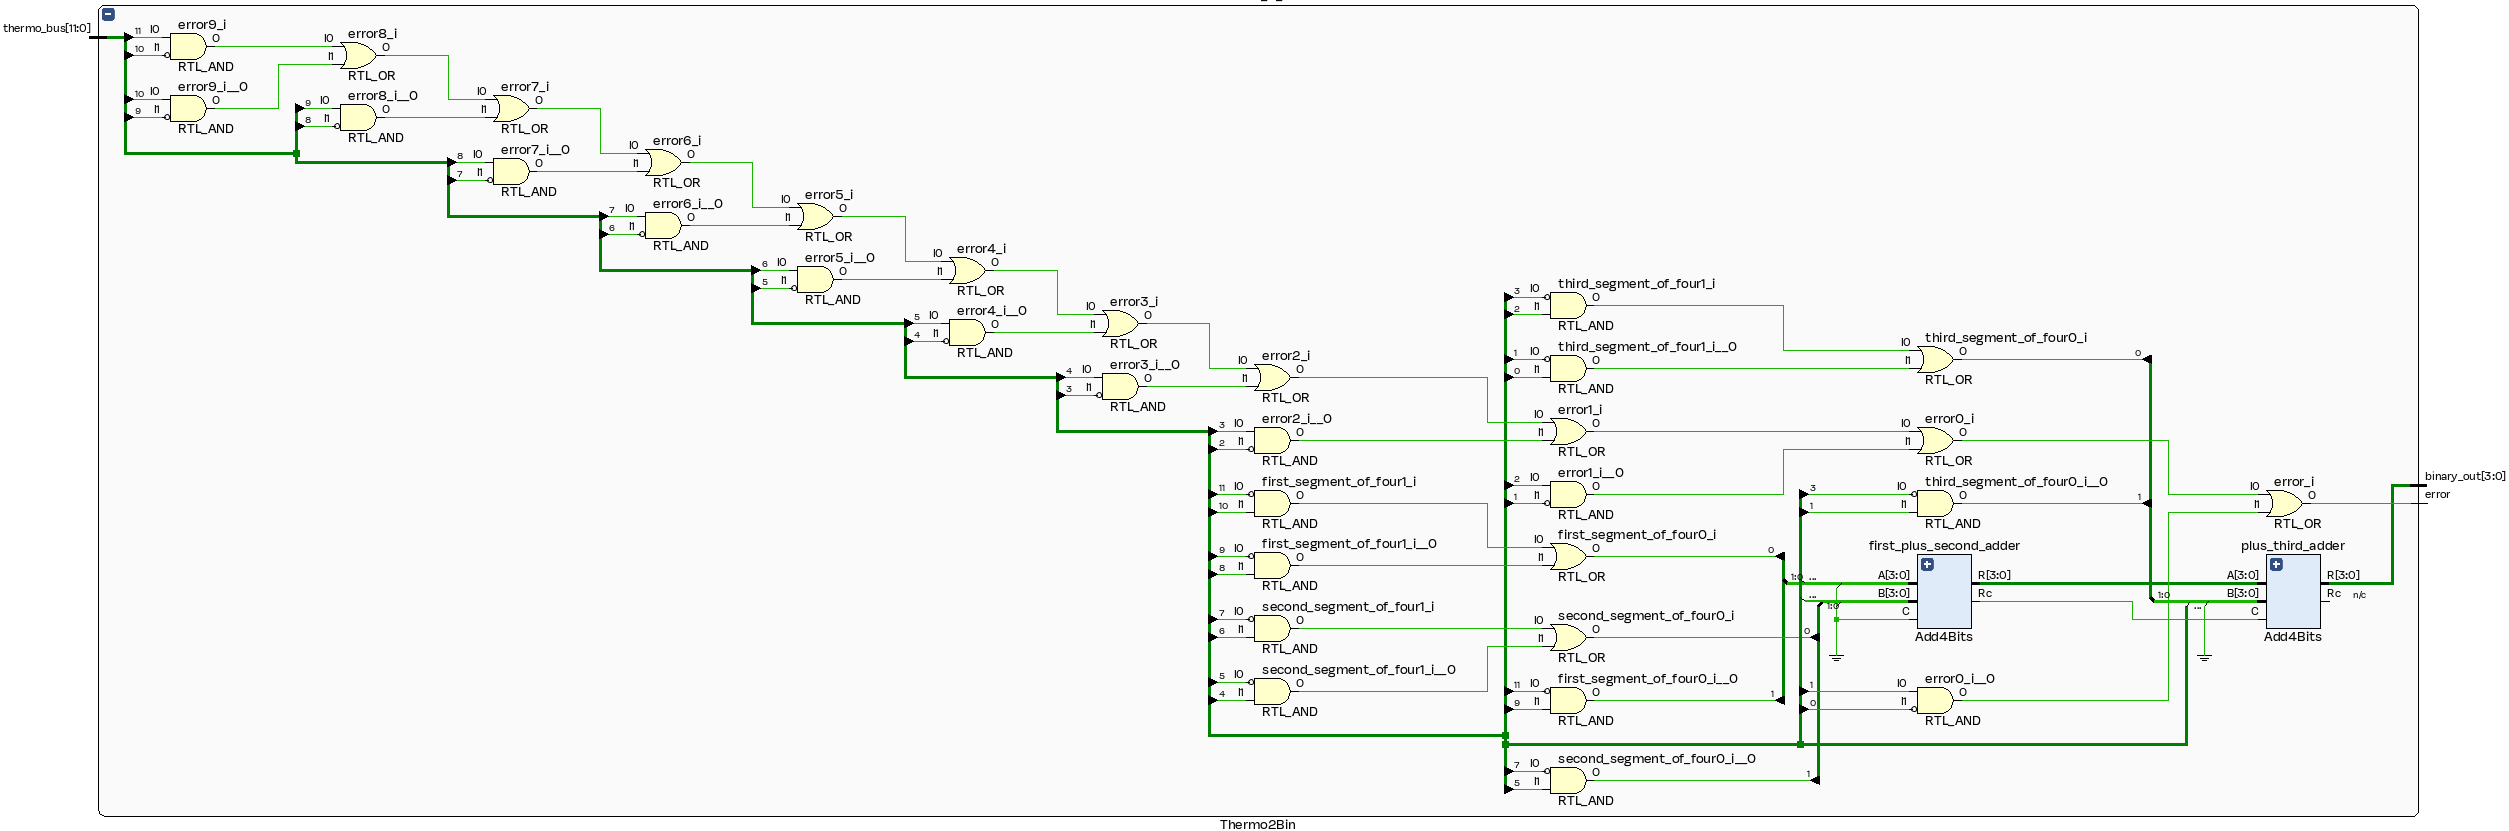
\includegraphics[width=.7\textwidth]{assets/img/schematic-thermo2bin.png}
	\caption{Module Thermo2bin}
\end{figure}

\begin{figure}[H]
	\centering
	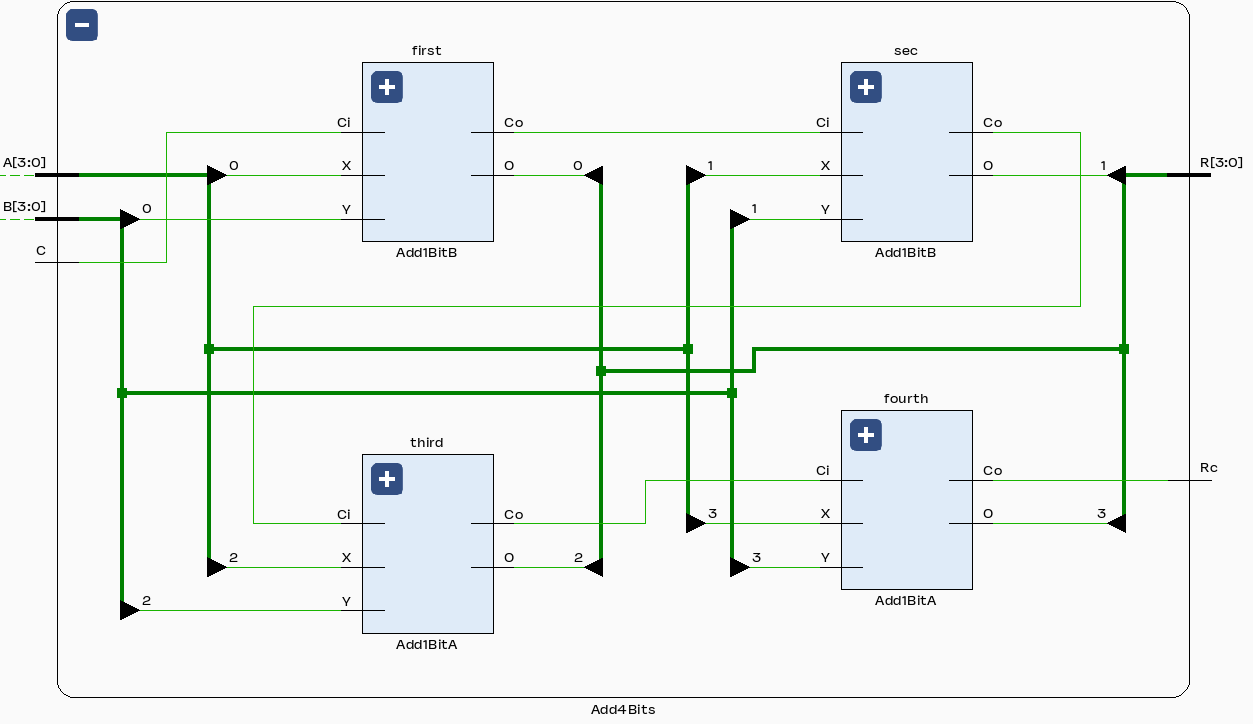
\includegraphics[width=.7\textwidth]{assets/img/schematic-add4bits.png}
	\caption{Module Add4Bits}
\end{figure}

\begin{figure}[H]
	\centering
	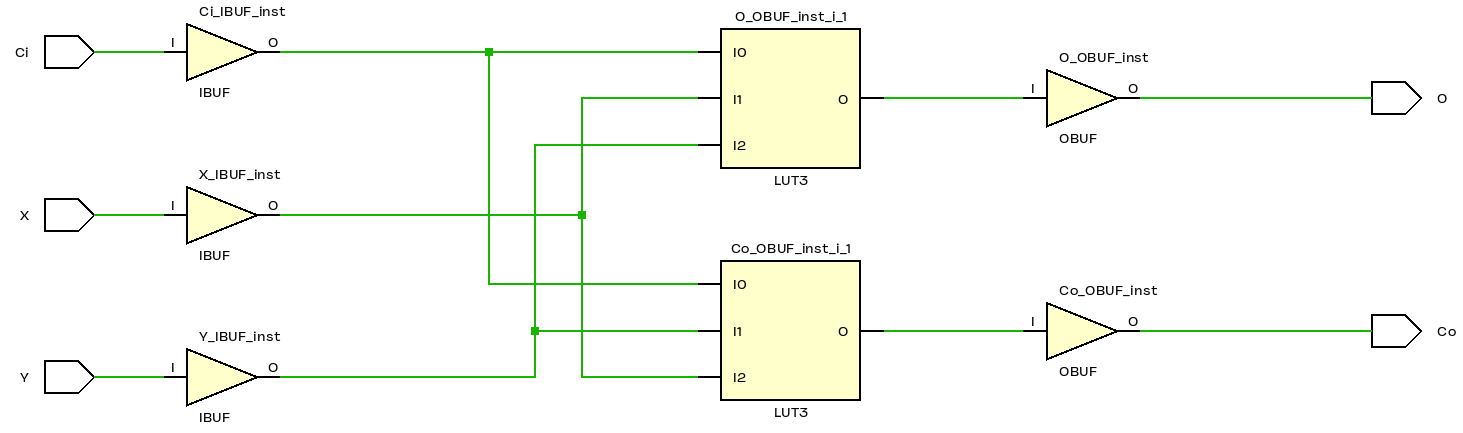
\includegraphics[width=.7\textwidth]{assets/img/schematic-add1bit.png}
	\caption{Module Add1Bit}
\end{figure}

\newpage
\section{Tables de Vérité et Karnaugh}

% \begin{figure}[H]
% \centering
% \begin{karnaugh-map}[4][4][1][$D$][$C$][$B$][$A$]
% \manualterms{
% 	0,1,2,3,
% 	4,5,6,7,
% 	8,9,10,11,
% 	12,13,14,15}
% \implicant{2}{10}
% \implicant{4}{13}
% \implicant{12}{10}
% \implicantedge{3}{2}{11}{10}
% \end{karnaugh-map}
% \caption{TEMPLATE NOT GOOD}
% \end{figure}


\begin{table}[H]
	\centering
	\caption{Table de vérité des Bits}
	\vspace{.2cm}
	\begin{tabular}{llllllll}
		\toprule
		A & B & C & D & E & F & G & H \\
		\midrule
		0 & 0 & 0 & 0 & 0 & 0 & 0 & 0 \\
		0 & 0 & 0 & 1 & 0 & 0 & 0 & 1 \\
		0 & 0 & 1 & 1 & 0 & 0 & 1 & 0 \\
		0 & 1 & 1 & 1 & 0 & 0 & 1 & 1 \\
		1 & 1 & 1 & 1 & 0 & 1 & 0 & 0 \\
		\bottomrule
	\end{tabular}

\end{table}

\begin{figure}[H]
\centering
\begin{karnaugh-map}[4][4][1][$D$][$C$][$B$][$A$]
\manualterms{
	0,1,X,0,
	X,X,X,1,
	X,X,X,X,
	X,X,X,0}
\implicant{1}{9}
\implicant{4}{6}
\end{karnaugh-map}
\caption{Karnaugh pour le bit $H$}
\end{figure}

\begin{figure}[H]
\centering
\begin{karnaugh-map}[4][4][1][$D$][$C$][$B$][$A$]
\manualterms{
	0,0,X,1,
	X,X,X,1,
	X,X,X,X,
	X,X,X,0}
\implicant{3}{6}
\end{karnaugh-map}
\caption{Karnaugh pour le bit $G$}
\end{figure}
